\documentclass[notitlepage]{math}
\usepackage{lipsum}
\title{Matrix Chap. 13} %Titre du fichie
\author{FireGhost} %Auteur du fichier

\usetikzlibrary{patterns,positioning, decorations, decorations.pathreplacing}
\begin{document}
\titre{Chapter 13: Matrix} %Titre du fichier .pdf
\UE{Matrix} %Nom de la UE

\fairetitre
\fairemarges
% subsubsubsection
\setcounter{secnumdepth}{4}

\titleformat{\paragraph}
{\normalfont\normalsize\bfseries}{\theparagraph}{1em}{}
\titlespacing*{\paragraph}
{0pt}{3.25ex plus 1ex minus .2ex}{1.5ex plus .2ex}

\newcommand{\MatrixDomaine}{\begin{smallmatrix}
    1 \leq i \leq n \\
    1 \leq j \leq p
\end{smallmatrix}}

%
\section{General approach}
\subsection{Definition}
\subsubsection{Definition of a matrix}
We call matrix of n rows and p columns any mapping in the following form:
\[\begin{matrix}
    \llbracket 1,n \rrbracket \times \llbracket 1,p \rrbracket & \rightarrow \mathbb{K} \\
    i,j &  a_{ij} 
\end{matrix}\]

We denote such maps as tables of n rows and p columns, and we write:

\[\begin{pmatrix}
    a_{11} & a_{12} & \cdots & a_{1p} \\
    a_{21} & a_{22} & \cdots & a_{2p} \\
    \vdots & \vdots & \ddots & \vdots \\
    a_{n1} & a_{n2} & \cdots & a_{np}
\end{pmatrix}\]

$\forall(i,j)\in \llbracket 1,n \rrbracket \times \llbracket 1,p \rrbracket$, we call $a_{ij}$ a coefficient of the matrix.
In this case coefficient if i-th row and j-th column.

\subsubsection{Notation}
We denote $M_{np}(\mathbb{K})$ the set of matrix of n rows and p columns with coefficient from $\mathbb{K}$.
\subsubsection{Examples}
%centering example

\[ A = \begin{pmatrix}
    1 & 4  \\
    2 & 5 \\
    3 & 6 
\end{pmatrix}\in M_{32}(\mathbb{R})\]
\[
B = \begin{pmatrix}
    i \\
    1 + i \\
    3
\end{pmatrix}\in M_{31}(\mathbb{C})\]

\subsection{Particular matrices}
Let $A \in M_{np}(\mathbb{K})$ then:
\subsubsection{Null matrix}
\begin{enumerate}
    \item  $\lbrack \forall (i,j) \in \llbracket 1,n \rrbracket \times \llbracket 1,p \rrbracket, a_{ij} = 0 \rbrack \Rightarrow \lbrack A = 0_{np} \rbrack$
    We say A is the null matrix $M_{np}(\mathbb{K})$.
\end{enumerate}
\paragraph{Example}
\[ A'=
\begin{pmatrix}
    0 & 0  \\
    0 & 0  \\
    0 & 0 
\end{pmatrix}\in M_{32}(\mathbb{R})\]

\subsubsection{Column matrix}
\begin{enumerate}
    \setcounter{enumi}{1}
    \item $B \in M_{np}(\mathbb{K})$ and $ p = 1 \Rightarrow $ B is a column matrix of n rows
\end{enumerate}
\paragraph{Example}
\[ B' = \begin{pmatrix}
    1 \\
    2 \\
    3
\end{pmatrix} \in M_{31}(\mathbb{R})\]

\subsubsection{Row matrix}
    \begin{enumerate}
        \setcounter{enumi}{2}
        \item $B \in M_{np}(\mathbb{K})$ and $ n = 1 \Rightarrow $ C is a row matrix of p columns
    \end{enumerate}
    \paragraph{Example}
    \[ C' = \begin{pmatrix}
        1 & 2 & 3
    \end{pmatrix} \in M_{13}(\mathbb{R})\]

\subsubsection{Square matrix}
    We call square matrix any matrix with same number of rows and columns.
    We denote $M_{n}(\mathbb{K})$ the set of square matrix of n rows and columns with coefficient from $\mathbb{K}$.
    \begin{enumerate}
        \setcounter{enumi}{3}
        \item $D \in M_{np}(\mathbb{K})$ and $ n = p \Rightarrow $ D is a square matrix denote $M_{n}(\mathbb{K})$
    \end{enumerate}
    \paragraph{Example}
    \[ D' = \begin{pmatrix}
        1 & 2 & 3 \\
        4 & 5 & 6 \\
        7 & 8 & 9
    \end{pmatrix} \in M_{3}(\mathbb{R})\]

\subsubsection{Diagonal matrix}
    \begin{enumerate}
        \setcounter{enumi}{4}
        \item $\forall E \in M_{n}(\mathbb{R})$, if $\forall (i,j) \in \llbracket 1,n \rrbracket ^2, i \neq j \Rightarrow a_{ij} = 0$ then we say E is a diagonal matrix
    \end{enumerate}
    \paragraph{Example}
    \[ E' = \begin{pmatrix}
        1 & 0 \\
        0 & 2
    \end{pmatrix} \in M_{2}(\mathbb{R})\]
    \[ E'' = \begin{pmatrix}
        1 & 0 & 0 \\
        0 & 2 & 0 \\
        0 & 0 & 3
    \end{pmatrix} \in M_{3}(\mathbb{R})\]
\subsubsection{Identity matrix}
    \begin{enumerate}
        \setcounter{enumi}{5}
        \item $\forall I_n \in M_{n}(\mathbb{R})$, if $\forall (i,j) \in \llbracket 1,n \rrbracket ^2, i \ne j \Rightarrow  a_{ij} = 0$ and $i = j \Rightarrow a_{ij} = 1$ then we say $I_n$ is a identity matrix
    \end{enumerate}
    \paragraph{Example}
    \[ I_n' = \begin{pmatrix}
        1 & 0 \\
        0 & 1
    \end{pmatrix} \in M_{2}(\mathbb{R})\]
    \[ I_n'' = \begin{pmatrix}
        1 & 0 & 0 \\
        0 & 1 & 0 \\
        0 & 0 & 1
    \end{pmatrix} \in M_{3}(\mathbb{R})\]



\subsubsection{Triangular matrix}
    \begin{enumerate}
        \setcounter{enumi}{5}
        \item $\forall F \in M_{n}(\mathbb{R})$, if $\forall (i,j) \in \llbracket 1,n \rrbracket ^2, i > j \Rightarrow a_{ij} = 0$ then we say F is a lower triangular matrix
        \item $\forall G \in M_{n}(\mathbb{R})$, if $\forall (i,j) \in \llbracket 1,n \rrbracket ^2, i < j \Rightarrow a_{ij} = 0$ then we say G is a upper triangular matrix
    \end{enumerate}
    \paragraph{Example}
    \[ F' = \begin{pmatrix}
        1 & 0 \\
        2 & 3
    \end{pmatrix} \in M_{2}(\mathbb{R})\]
    \[ G' = \begin{pmatrix}
        1 & 2 \\
        0 & 3
    \end{pmatrix} \in M_{2}(\mathbb{R})\]

\subsection{Transposed matrix}
    \subsubsection{Definition}
        Let $A \in M_{np}(\mathbb{K})$. We call transposed matrix of A (or A transpose) a matrix B from $M_{pn}(\mathbb{K})$ such as:
        \[ \forall (i,j) \in \llbracket 1,n \rrbracket \times \llbracket 1,p \rrbracket, a_{ij} = b_{ji}\]
    \subsubsection{Notation}
    We denote B as ${}^t \! A$
    \subsubsection{Example}
    
    \[ A = \begin{pmatrix}
        1 & 2 & 3 \\
        4 & 5 & 6
    \end{pmatrix} \in M_{23}(\mathbb{R})\]
    \[ {}^t \! A = \begin{pmatrix}
        1 & 4 \\
        2 & 5 \\
        3 & 6
    \end{pmatrix} \in M_{32}(\mathbb{R})\]


\subsection{Symmetric matrix}
    \subsubsection{Symmetric}
        If $ {}^t \! A = A $ then we say A is symmetric
        \paragraph{Example}
        \[ A = \begin{pmatrix}
            1 & 2 & 3 \\
            2 & 4 & 5 \\
            3 & 5 & 6
        \end{pmatrix} = {}^t \! A = 
        \begin{pmatrix}
            1 & 2 & 3 \\
            2 & 4 & 5 \\
            3 & 5 & 6
        \end{pmatrix}
            \in M_{3}(\mathbb{R})\]
    \subsubsection{Anti-Symmetric}
        If $ {}^t \! A = -A $ then we say A is Anti-symmetric
        \paragraph{Example}
        \[ A = \begin{pmatrix}
            0 & -2 & 3 \\
            2 & 0 & -5 \\
            -3 & 5 & 0
        \end{pmatrix} = -{}^t \! A = 
        \begin{pmatrix}
            0 & 2 & -3 \\
            -2 & 0 & 5 \\
            3 & -5 & 0
        \end{pmatrix}
            \in M_{3}(\mathbb{R})\]
\section{Operations on matrices}
\subsection{Addition and external product}
\subsubsection{Definition}
\begin{enumerate}
    \item We call internal operation in $M_{np}(\mathbb{K})$ denoted $\oplus$ "internal addition" the one defined as follows:
    \[ \forall A,B \in M^2_{np}(\mathbb{K}),  A + B = (a_{ij} + b_{ij})_{\MatrixDomaine}\]
    \[ \text{Where } A = {a_{ij}}_{\MatrixDomaine} \text{ and } B = {b_{ij}}_{\MatrixDomaine}\]
    \item We call "external multiplication" or "multiplication by a scalar" the one defined as follows:
    \[ \forall A \in M_{np}(\mathbb{K}), \forall \alpha \in \mathbb{K}, \alpha A = (\alpha a_{ij})_{\MatrixDomaine}\]
\end{enumerate}
\paragraph{Example}
\begin{align*}
    (A,B) &\in M_{2,3}(\mathbb{R})^2 \quad A = \begin{pmatrix}
        1 & 2 & 3 \\
        4 & 5 & 6
    \end{pmatrix} \text{ and } B = \begin{pmatrix}
        7 & 8 & 9 \\
        10 & 11 & 12
    \end{pmatrix} \\
    A + B & = \begin{pmatrix}
        1 + 7 & 2 + 8 & 3 + 9 \\
        4 + 10 & 5 + 11 & 6 + 12
    \end{pmatrix} = \begin{pmatrix}
        8 & 10 & 12 \\
        14 & 16 & 18
    \end{pmatrix} \\
    \alpha = 3,& \quad \alpha A = \begin{pmatrix}
        3 \times 1 & 3 \times 2 & 3 \times 3 \\
        3 \times 4 & 3 \times 5 & 3 \times 6
    \end{pmatrix} = \begin{pmatrix}
        3 & 6 & 9 \\
        12 & 15 & 18
    \end{pmatrix}
\end{align*}
\paragraph{Proposition}
\[(M_{np}, \oplus, \cdot) \text{ is a vector space over } \mathbb{K}\]
\subsubsection{Elementary matrix}
For $(n,p) \in \mathbb{N}^2, (i,j) \in \llbracket 1,n \rrbracket \times \llbracket 1,p \rrbracket;$ We denote $E_{ij}$ the matrix from $M_{np}(\mathbb{K})$
such that the $ij$-th coefficient is $1$ and all other coefficient are $0$.
\[ E_{ij} \text{ are called elementary matrix}\]
\paragraph{Example}
\begin{align*}
    E_{11} & = \begin{pmatrix}
        1 & 0 \\
        0 & 0 \\
    \end{pmatrix} \\
    E_{22} & = \begin{pmatrix}
        0 & 0 & 0 \\
        0 & 1 & 0 \\
        0 & 0 & 0
    \end{pmatrix} \\
    E_{33} & = \begin{pmatrix}
        0 & 0 & 0 \\
        0 & 0 & 0 \\
        0 & 0 & 1
    \end{pmatrix}
\end{align*}
\subsubsection{Proposition}
\begin{enumerate}
    \item $(E_{ij})_{\MatrixDomaine}$ is a basis of $M_{np}(\mathbb{K})$
    \item $dim((E_{ij})_{\MatrixDomaine}) = np$ \\
    Ex: $M_{2}(\mathbb{R})$ a $(\mathbb{K})$-VS: B = $\left( 
        \begin{pmatrix}
            1 & 0 \\
            0 & 0
        \end{pmatrix},
        \begin{pmatrix}
            0 & 1 \\
            0 & 0
        \end{pmatrix},
        \begin{pmatrix}
            0 & 0 \\
            1 & 0
        \end{pmatrix},
        \begin{pmatrix}
            0 & 0 \\
            0 & 1
        \end{pmatrix}
    \right)$\\
    B is a Standard basis of $M_{2}(\mathbb{R})$, $dim(M_2(\mathbb{R})) = 2^2 = 4$
\end{enumerate}
\subsection{Internal product}
\subsubsection{Definition}
Let $(n,p,q) \in \mathbb{N}^3$ and $A = {a_{ij}}_{\MatrixDomaine} \in M_{np}(\mathbb{K}), B = {b_{ij}}_{\begin{smallmatrix}1 \leq i \leq p \\1 \leq j \leq q\end{smallmatrix}} \in M_{pq}(\mathbb{K})$.
We call product of $A$ and $B$ the matrix $C$ form $M_{nq}(\mathbb{K})$ such that:
\[ \forall (i,j) \in \llbracket 1,n \rrbracket \times \llbracket 1,q \rrbracket, c_{ij} = \sum_{k=1}^{p} a_{ik}b_{kj}\]

\paragraph{Example}
\[
    A = \begin{pmatrix}
        1 & 2 & 3 \\
        \color{red} 4 & \color{red}5 & \color{red}6
    \end{pmatrix} \in M_{2,3}(\mathbb{R}) \quad \text{ and } \quad B = \begin{pmatrix}
        1 & 0 & \color{red}1 & 3 \\
        0 & 0 & \color{red}2 & 4 \\
        0 & 0 & \color{red}1 & 0
    \end{pmatrix} \in M_{3,4}(\mathbb{R}) \]
    \[C = A \cdot B = \begin{pmatrix}
        1 & 0 & 8 & 11 \\
        4 & 0 & \color{red}20 & 32
    \end{pmatrix} \in M_{2,4}(\mathbb{R})\]
    \[ C_{2,3} = 4 \times 1 + 5 \times 2 + 6 \times 1 = 20 \] 
\subsubsection{Remarks}
\begin{enumerate}[label=\protect\circled{R\arabic*}]
    \item If $A,B$ two matrices: we only can multiply $A$ by $B$ if the number of column of $A$ is equal to the number of row of $B$.
    \item $AB$ can exists but $BA$ not or the other way around.
        \paragraph{Example}
        \[A = \begin{pmatrix}
            1 & 2 & 3\\
            4 & 5 & 6
        \end{pmatrix} \cdot B = \begin{pmatrix}
            1 \\
            2 \\
            3
        \end{pmatrix} \Rightarrow M_{2,1}(\mathbb{R}) \text{, and exists but } BA \text{ does not exists}\]
    \item In the \fbox{General case}, where $AB$ and $BA$ exists:\\
    {\color{red}{\fbox{ \color{black}AB $\neq$ BA }}} (multiplication of matrix is not commutative)\\
    When $AB = BA$ we say $A$ and $B$ commute. 
\end{enumerate}
\subsection{Properties of matrix calculus}
\subsubsection{Properties}
\begin{enumerate}
    \item Let $A,B$ two matrices such that $AB$ exists. \\
    We can have $AB = 0$ and ($A \neq 0$ or $B \neq 0$)\\
    \[ \text{If } A = 0 \text{ or } B = 0 \text{ then } AB = 0 \]
    \[ AB = 0 \nRightarrow A = 0 \text{ or } B = 0 \]
    \paragraph{Example}
    \[\begin{pmatrix}
        1 & 1 \\
        1 & 1 
    \end{pmatrix} \cdot \begin{pmatrix}
        -2 & 3 \\
        2 & -3 
    \end{pmatrix} = \begin{pmatrix}
        0 & 0 \\
        0 & 0
    \end{pmatrix}\]
    \item $(n,p,q,r) \in \mathbb{N}^4$ and let $ (A,B,C) \in M_{np}(\mathbb{K}) \times M_{pq}(\mathbb{K}) \times M_{qr}(\mathbb{K})$\\
    \[ A \cdot (B \cdot C) = (A \cdot B) \cdot C \otimes \text{ is commutative}\] 
    \item $(A,B,C) \in M_{np}(\mathbb{K}) \times M_{pq}^2(\mathbb{K})$
    \[ A \cdot (B + C) = A \cdot B + A \cdot C\]
    $\otimes$ (Matrices multiplication) is distributive over matrix addition ($\oplus$). 
    \item $ A \in M_{np}(\mathbb{K})$ and $B \in M_{pq}(\mathbb{K})$ and $ \lambda \in \mathbb{K}$\\
    \[ \lambda \cdot (A \cdot B) = A \cdot \lambda \cdot B = A \cdot B \cdot \lambda \] 
\end{enumerate}
\subsubsection{Case of Square Matrices}
\begin{enumerate}
    \item \[ \forall A \in M_{n}(\mathbb{K}), A \cdot I_n  = I_n \cdot A = A \]
    \item Let $(A,B) \in M_{n}(\mathbb{K})^2$, such that {\color{red}{\fbox{\color{black}$ AB = BA $}}} Then:
    \[ (A+B)^n { \color{red}{\fbox{\color{black}$ = $}}} \sum_{k=0}^{n} \binom{n}{k} A^k B^{n-k} \]
    By convention, $A^0 = B^0 = I_n$\\
    \item \[ \forall (A,B) \in M_{n}(\mathbb{K})^2, {} ^ t (A \cdot B) = {} ^t A \cdot {} ^ t B \]
\end{enumerate}
\subsection{Inverse of a matrix}
\subsubsection{Definition}
Let $A \in M_{n}(\mathbb{K})$ we say that $A$ is invertible if:
\[  \exists B \in M_{n}(\mathbb{K}), AB = BA = I_n \]
Then we say that $B$ is the inverse of $A$ and denote $B = A^{-1}$ $\quad$ (B is unique)
Hence we have (in case of A invertible): $A \cdot A^{-1} = A^{-1} \cdot A = I_n$
\subsubsection{Notation}
The set of invertible matrices of $M_{n}(\mathbb{K})$ is denoted $GL_n(\mathbb{K})$
\subsubsection{How to find the inverse of a matrix}
We will use the following system:
Where $A \in M_{n}(\mathbb{K}), (U,V) \in M_{n,1}(K)^2$:
\[A \cdot U = V  \]
By solving this system (Gauss elimination algorithm) when $A$ is invertible, we will have:
\[ U = A^{-1} \cdot V \]
\paragraph{Example}
\begin{align*}
        A = \begin{pmatrix}
        1 & 0 & 1 \\
        0 & 1 & 1 \\
        1 & 1 & 0 
        \end{pmatrix} 
        A \cdot X = U \Rightarrow& 
        \begin{pmatrix}
            1 & 0 & 1 \\
            0 & 1 & 1 \\
            1 & 1 & 0
        \end{pmatrix} \cdot \begin{pmatrix}
            a \\
            b \\
            c
        \end{pmatrix} = \begin{pmatrix}
            x \\
            y \\
            z
        \end{pmatrix} \\
        \Longleftrightarrow & 
        \begin{pmatrix}
            \circled{1} & 0 & 1 \\
            0 & 1 & 1 \\
            0 & 1 & -1
        \end{pmatrix}
        =
        \begin{pmatrix}
            x \\
            y \\
            z - x
        \end{pmatrix} \\
        \Longleftrightarrow &
        \begin{pmatrix}
            1 & 0 & 1 \\
            0 & 1 & 1 \\
            0 & 0  & -2
        \end{pmatrix} = 
        \begin{pmatrix}
            x \\
            y \\
            z - x - y
        \end{pmatrix} \\
        \Longleftrightarrow &
        \begin{pmatrix}
            2 & 0 & 0 \\
            0 & 2 & 0 \\
            0 & 0  & -2
        \end{pmatrix} =
        \begin{pmatrix}
            x - y + z \\
            -x + y + z \\
            z - x - y
        \end{pmatrix} \\
        \Longleftrightarrow &
        \begin{pmatrix}
            1 & 0 & 0 \\
            0 & 1 & 0 \\
            0 & 0  & 1
        \end{pmatrix} = 
        \begin{pmatrix}
            \frac{x - y + z}{2} \\
            \frac{-x + y + z}{2} \\
            \frac{x + y - z}{2}
        \end{pmatrix} \\
        \Longleftrightarrow &
        \begin{pmatrix}
            a \\
            b \\
            c
        \end{pmatrix} =
        \begin{pmatrix}
            \frac{1}{2} & -\frac{1}{2} & \frac{1}{2} \\ 
            -\frac{1}{2} & \frac{1}{2} & \frac{1}{2} \\
            \frac{1}{2} & \frac{1}{2} & -\frac{1}{2}
        \end{pmatrix} \cdot
        \begin{pmatrix}
            x \\
            y \\
            z
        \end{pmatrix} \\
        A ^{-1} = \begin{pmatrix}
            \frac{1}{2} & -\frac{1}{2} & \frac{1}{2} \\ 
            -\frac{1}{2} & \frac{1}{2} & \frac{1}{2} \\
            \frac{1}{2} & \frac{1}{2} & -\frac{1}{2}
        \end{pmatrix}
\end{align*}
\section{Matrices of Linear Maps}
\subsection{Definition and examples}
\subsubsection{Definition}
Let $f \in \mathcal{L}(E,F)$, $E$ and $F$ finite dimensional $\mathbb{K}$-vector spaces such that:
$dim (E) = p$ and $dim (F) = n$ where $(p,n) \in \mathbb{N}^2$ and $B = (e_1,e_2,\dots,e_n)$ basis of E and $B' = (e_1',e_2',\dots,e_n')$ basis of F
\[ \forall U \in E, \exists ! (\lambda_1, \lambda_2, \dots, \lambda_n) \in \mathbb{K}^p, \quad U=\sum_{i=1}^{p} \lambda_i e_i' \]
We say $\begin{pmatrix} U_1 \\ U_2 \\ \vdots \\ U_n \end{pmatrix}$ is the column matrix of coordinates $A \cdot U$ in $B$.
\subsubsection{Example}
Let $E = \mathbb{R}^2$, $U = {\begin{pmatrix} 1 \\ 2 \end{pmatrix}}_B$ with $B = (\begin{pmatrix} 1 \\ 0 \end{pmatrix}, \begin{pmatrix} 0 \\ 1 \end{pmatrix})$ and $B' = (\begin{pmatrix} 1 \\ 1 \end{pmatrix}, \begin{pmatrix} 1 \\ 0 \end{pmatrix})$Then:
\[U = {\begin{pmatrix} 2 \\ 1 \end{pmatrix}}_B = {\begin{pmatrix} 1 \\ 1 \end{pmatrix}}_B + {\begin{pmatrix} 1 \\ 0 \end{pmatrix}}_B \Rightarrow U = {\begin{pmatrix} 1 \\ 1 \end{pmatrix}}_{B'}\]
\subsubsection{Definition}
We call matrix of $f \in \mathcal{L}(E,F)$ with respect to basis $B$ and $B'$ denoted $Mat_{BB'}(f)$ the matrix whose $j-th$ column is composed of the coordinates of $f(e_j)$ in $B'$, for all j from $\llbracket 1,p \rrbracket$.
This is a matrix of $p$ columns and $n$ rows:
\[\begin{pmatrix}
    a_{11} & a_{12} & \cdots & a_{1p} \\
    a_{21} & a_{22} & \cdots & a_{2p} \\
    \vdots & \vdots & \ddots & \vdots \\
    a_{n1} & a_{n2} & \cdots & a_{np}
\end{pmatrix}, \forall j \in \llbracket 1,p \rrbracket, f(e_j) = {\begin{pmatrix} a_{1j} \\ a_{2j} \\ \vdots \\ a_{nj} \end{pmatrix}}_{B'} = \sum_{i=1}^{n} a_{ij} e_i\]
\subsubsection{Example}
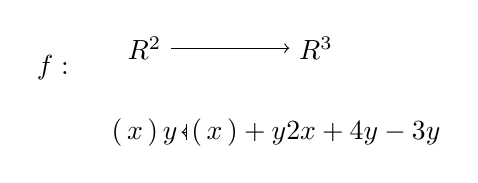
\begin{tikzpicture}[node distance=1mm]
    \node (functionName) at (0, -0.5) {$f:$};

    \node[above right = -0.3cm and 0.5cm of functionName] (domain) {$\mathbb{R}^2$};
    \node[right = 1.5cm of domain] (codomain) {$\mathbb{R}^3$};
    \node[below = 5mm of domain] (element) {$\begin{pmatrix} x \\ y \end{pmatrix}$};
    \node at (element-|codomain) (image) {$\begin{pmatrix} x + y \\ 2x + 4y \\ -3y \end{pmatrix}$};
    \draw[->] (domain) -- (codomain);
    \draw[|->] (element) -- (image) ;
\end{tikzpicture}

     

\begin{enumerate}[label=\protect\circled{\arabic*}]
    \item basis for the domain ($\mathbb{R}^2$): B = ($\begin{pmatrix} 1 \\ 0 \end{pmatrix}, \begin{pmatrix} 0 \\ 1 \end{pmatrix})$\\
    basis for the codomain ($\mathbb{R}^3$): $B' = (\begin{pmatrix} 1 \\ 0 \\ 0 \end{pmatrix}, \begin{pmatrix} 0 \\ 1 \\ 0 \end{pmatrix}, \begin{pmatrix} 0 \\ 0 \\ 1 \end{pmatrix}$)

    \item $\begin{pmatrix}
        x + y \\
        2x + 4y \\
        -3y
    \end{pmatrix} \Rightarrow \begin{cases}
        f(\begin{pmatrix} 1 \\ 0 \end{pmatrix}) = {\begin{pmatrix} 1 \\ 2 \\ 0 \end{pmatrix}}_{B'} \\
        f(\begin{pmatrix} 0 \\ 1 \end{pmatrix}) = {\begin{pmatrix} 1 \\ 4 \\ -3 \end{pmatrix}}_{B'}
    \end{cases}$
    \item \[\forall U \in \mathbb{R}^2, U = x \cdot \begin{pmatrix} 1 \\ 0 \end{pmatrix} + y \cdot \begin{pmatrix} 0 \\ 1 \end{pmatrix} \Rightarrow f(U) = x \cdot f \begin{pmatrix} 1 \\ 0 \end{pmatrix} + y \cdot f \begin{pmatrix} 0 \\ 1 \end{pmatrix}\]
    \[ \Rightarrow \begin{pmatrix}
        1 & 1 \\
        2 & 4 \\
        0 & -3
    \end{pmatrix}\]
    \[ \Rightarrow \begin{pmatrix}
        1 & 1 \\
        2 & 4 \\
        0 & -3
    \end{pmatrix} \cdot \begin{pmatrix}
        1 \\
        -1 
    \end{pmatrix} = \begin{pmatrix}
        0 \\
        -2 \\
        3
    \end{pmatrix}\]
    \[ \text{so } f \left(\begin{pmatrix} 1 \\ -1 \end{pmatrix}\right) = \begin{pmatrix} 0 \\ -2 \\ 3 \end{pmatrix}\]
\end{enumerate}
\subsection{Matrix interpretation of Linear Transformation}
\subsubsection{Proposition}
Let $E$ and $F$ two finite dimensional $\mathbb{K}$-VS, $B$ and $B'$ bases of respectively $E$ and $F$. Let $U \in E$ and $f \in \mathcal{L}(E,F)$.
Then:
\[ Mat_{B'}(f(u)) = Mat_{BB'}(f) \cdot Mat_{B}(u)\]
\subsubsection{Example}
With the same function as before: \\
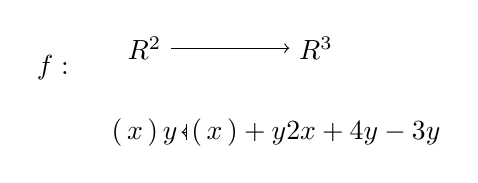
\begin{tikzpicture}[node distance=1mm]
    \node (functionName) at (0, -0.5) {$f:$};

    \node[above right = -0.3cm and 0.5cm of functionName] (domain) {$\mathbb{R}^2$};
    \node[right = 1.5cm of domain] (codomain) {$\mathbb{R}^3$};
    \node[below = 5mm of domain] (element) {$\begin{pmatrix} x \\ y \end{pmatrix}$};
    \node at (element-|codomain) (image) {$\begin{pmatrix} x + y \\ 2x + 4y \\ -3y \end{pmatrix}$};
    \draw[->] (domain) -- (codomain);
    \draw[|->] (element) -- (image) ;
\end{tikzpicture}\\
And with the same basis as before:
$B = (\begin{pmatrix} 1 \\ 0 \end{pmatrix}, \begin{pmatrix} 0 \\ 1 \end{pmatrix})$ and $B' = (\begin{pmatrix} 1 \\ 0 \\ 0 \end{pmatrix}, \begin{pmatrix} 0 \\ 1 \\ 0 \end{pmatrix}, \begin{pmatrix} 0 \\ 0 \\ 1 \end{pmatrix})$ \\

And with $u = \begin{pmatrix} 1 \\ 2 \end{pmatrix}$ we have:
\begin{align*}
    Mat_{B'}(f(u)) &= Mat_{B'}(f) \cdot Mat_{B}(u) \\
     &= \begin{pmatrix}
        1 & 1 \\
        2 & 4 \\
        0 & -3
    \end{pmatrix} \cdot \begin{pmatrix}
        1 \\
        2
    \end{pmatrix} 
    = \begin{pmatrix}
        3 \\
        10 \\
        -6
    \end{pmatrix} = f(u)
\end{align*}
\subsection{Matrix of g o f}
\subsubsection{Proposition}
Let $E,F$ and $G$ three finite dimensional $\mathbb{K}$-VS, and $B,B',B''$ bases of respectively $E,F$ and $G$. Considering $f \in \mathcal{L}(E,F)$ and $g \in \mathcal{L}(F,G)$, we have $g \circ  f \in \mathcal{L}(E,G)$ and:
\[ Mat_{BB''}(g \circ f) = Mat_{B'B''}(g) \cdot Mat_{BB'}(f)\]
\subsubsection{Example}
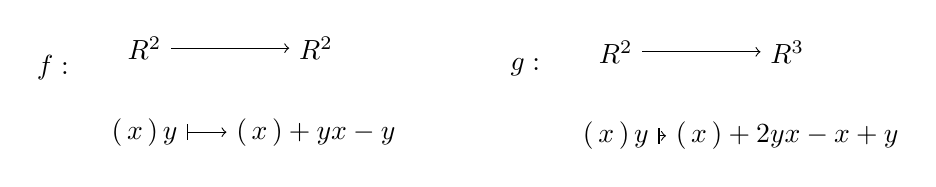
\begin{tikzpicture}[node distance=1mm]
    \node (functionName) at (0, -0.5) {$f:$};
    \node (functionName2) at (6, -0.5) {$g:$};
    
    \node[above right = -0.3cm and 0.5cm of functionName] (domain) {$\mathbb{R}^2$};
    \node[above right = -0.3cm and 0.5cm of functionName2] (domain2) {$\mathbb{R}^2$};

    \node[right = 1.5cm of domain] (codomain) {$\mathbb{R}^2$};
    \node[right = 1.5cm of domain2] (codomain2) {$\mathbb{R}^3$};

    \node[below = 5mm of domain] (element) {$\begin{pmatrix} x \\ y \end{pmatrix}$};
    \node[below = 5mm of domain2] (element2) {$\begin{pmatrix} x \\ y \end{pmatrix}$};

    \node at (element-|codomain) (image) {$\begin{pmatrix} x + y \\ x - y \end{pmatrix}$};
    \node at (element2-|codomain2) (image2) {$\begin{pmatrix} x + 2y \\ x \\ -x + y \end{pmatrix}$};

    \draw[->] (domain) -- (codomain);
    \draw[->] (domain2) -- (codomain2);
    \draw[|->] (element) -- (image) ;
    \draw[|->] (element2) -- (image2) ;

\end{tikzpicture}
And with the following basis:
$B = (\begin{pmatrix} 1 \\ 0 \end{pmatrix}, \begin{pmatrix} 0 \\ 1 \end{pmatrix})$ and $B' = (\begin{pmatrix} 1 \\ 0 \\ 0 \end{pmatrix}, \begin{pmatrix} 0 \\ 1 \\ 0 \end{pmatrix}, \begin{pmatrix} 0 \\ 0 \\ 1 \end{pmatrix})$ \\
\[ Mat_B(f)= \begin{pmatrix}
        1 & 1 \\
        1 & -1
    \end{pmatrix} \quad \text{and} \quad Mat_{BB'}(g)=\begin{pmatrix}
        1 & 2  \\
        1 & 0  \\
        -1 & 1
    \end{pmatrix}\]
    \[ \forall X = \begin{pmatrix} x \\ y \end{pmatrix} \in \mathbb{R}^2, \quad g \circ f(X) = g(f(X)) = g \left(\begin{pmatrix}
        1 & 1 \\
        1 & -1
    \end{pmatrix} \cdot \begin{pmatrix}
        x \\
        y
    \end{pmatrix} \right)\]
    \[ g \circ f(X) =
        \begin{pmatrix}
        1 & 2  \\
        1 & 0  \\
        -1 & 1
    \end{pmatrix} \cdot \begin{pmatrix}
        1 & 1 \\
        1 & -1
    \end{pmatrix} \cdot \begin{pmatrix}
        x \\
        y
    \end{pmatrix} = \begin{pmatrix}
        3 & -1 \\
        1 & 1 \\
        0 & -2 
    \end{pmatrix} \cdot \begin{pmatrix}
        x \\
        y
    \end{pmatrix} \]

\subsection{Matrix of a bijection}
\subsubsection{Proposition}
Let $E$ and $F$ two $\mathbb{K}$-VS of same dimension. $B$ a bases of $E$ and $B'$ a bases of $F$. Let $f \in \mathcal{L}(E,F)$ Then:
\[ f \text{ bijective } \Longleftrightarrow Mat_{BB'}(f) \text{ is invertible }\]
\subsubsection{Example}
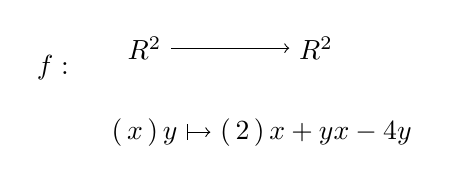
\begin{tikzpicture}[node distance=1mm]
    \node (functionName) at (0, -0.5) {$f:$};

    \node[above right = -0.3cm and 0.5cm of functionName] (domain) {$\mathbb{R}^2$};
    \node[right = 1.5cm of domain] (codomain) {$\mathbb{R}^2$};
    \node[below = 5mm of domain] (element) {$\begin{pmatrix} x \\ y \end{pmatrix}$};
    \node at (element-|codomain) (image) {$\begin{pmatrix} 2x + y \\ x - 4y \end{pmatrix}$};
    \draw[->] (domain) -- (codomain);
    \draw[|->] (element) -- (image) ;
\end{tikzpicture}\\
To find if $f$ is bijective, we have to show that $f$ is surjective or injective, because $f$ is a endomorphism. \\
with: $B = \left(\begin{pmatrix} 1 \\ 0 \end{pmatrix}, \begin{pmatrix} 0 \\ 1 \end{pmatrix}\right)$ 
and $Mat(f) = \begin{pmatrix} 2 & 1 \\
        1 & -4
    \end{pmatrix}$ \\
To prove $f$ is injective, we have to show that $ker (f) = \left\{ 0_{\mathbb{R}^2} \right\}$
\begin{align*}   
    f(X)  = \begin{pmatrix} 0 \\ 0 \end{pmatrix} &\Longleftrightarrow \begin{pmatrix} 2 & 1 \\
        1 & -4
    \end{pmatrix} \cdot \begin{pmatrix} x \\ y \end{pmatrix} = \begin{pmatrix} 0 \\ 0 \end{pmatrix} \\
    &\Longleftrightarrow
    \begin{pmatrix}
        2 & 1 \\
        0 & -9
    \end{pmatrix} \text{ : } \begin{pmatrix} 0 \\ 0 \end{pmatrix} \\
    &\Longleftrightarrow x = y = 0 \Rightarrow S = \left\{ 0_{\mathbb{R}^2} \right\} \\ 
    &\Leftrightarrow f \text{ is injective so } f \text{ is bijective}
\end{align*}
Lets find the inverse of $f$, using two methods: \\
\paragraph{Method 1: Gauss elimination algorithm}
\begin{align*}
    &\begin{pmatrix} 2 & 1 \\
            1 & -4
    \end{pmatrix} \cdot \begin{pmatrix} x \\ y \end{pmatrix} = \begin{pmatrix} a \\ b \end{pmatrix} \\
    &\Longleftrightarrow \begin{pmatrix} 2 & 1 \\
                 0 & -9 
    \end{pmatrix} \text{ : } \begin{pmatrix} a \\ 2b-a \end{pmatrix} \\
    &\Longleftrightarrow \begin{pmatrix} 18 & 0 \\
             0 & -9
    \end{pmatrix} \text{ : } \begin{pmatrix} 8a  + 2b\\ 2b-a \end{pmatrix} \\
    &\Longleftrightarrow \begin{pmatrix} 1 & 0 \\ 0 & 1 \end{pmatrix} \cdot \begin{pmatrix} x \\ y \end{pmatrix} 
    = \begin{pmatrix} \frac{4a + b}{9} \\ \frac{a-2b}{9} \end{pmatrix} = \frac{1}{9} \begin{pmatrix} 4a + b \\ a-2b \end{pmatrix} \\
    &\Longleftrightarrow \begin{pmatrix} x \\ y \end{pmatrix} = \frac{1}{9} \begin{pmatrix} 4& 1 \\ 1 & -2 \end{pmatrix} \cdot \begin{pmatrix} a \\ b \end{pmatrix} \\
\end{align*}
\paragraph{Method 2: System, Gauss-Jordan}


Operations on left must be done also on right:
\begin{align*}
    \left( \begin{array}{cc|cc}
        2 & 1 & 1 &  0 \\
        1 & -4 & 0 & 1 \\
    \end{array}\right)  & \Longleftrightarrow 
    \left( \begin{array}{cc|cc}
        2 & 1 & 1 &  0 \\
        0 & -9 & -1 & 2 \\
    \end{array}\right) \\
    &\Longleftrightarrow 
    \left( \begin{array}{cc|cc}
        18 & 0 & 8 &  2 \\
        0 & -9 & -1 & 2 \\
    \end{array}\right)  \\
    &\Longleftrightarrow 
    \left( \begin{array}{cc|cc}
        1 & 0 & \frac{4}{9} &  \frac{1}{9} \\
        0 & 1 & -\frac{1}{9} & -\frac{2}{9} \\
    \end{array}\right) 
\end{align*}
With both methods we have:
    
    
    \[ \left[ Mat_{B}(f) \right]^{-1} = \frac{1}{9} \begin{pmatrix} 4& 1 \\ 1 & -2 \end{pmatrix} \]
    
    


\subsubsection{Proposition}
%if f bij then Mat(f)^-1 = Mat(f^-1)
Let $E$ and $F$ two $\mathbb{K}$-VS of same dimension. $B$ a bases of $E$ and $B'$ a bases of $F$. Let $f \in \mathcal{L}(E,F)$ Then:
\[ f \text{ bijective } \Longleftrightarrow Mat_{BB'}(f) \text{ is invertible }\]
And in this case we have:
\[ \left[Mat_{BB'}(f)\right]^{-1} = Mat_{BB'}(f^{-1})\]
\subsubsection{Examples}
\paragraph{Example 1}
$A = \begin{pmatrix} 1 & 1 & 0 \\ 1 & 0 & 1 \\ 1 & 1 & 1 \end{pmatrix}$ \\
\circled{1} Is $A$ invertible, compute the inverse of $A$ \\
\begin{align*}
    & \left( \begin{array}{ccc|ccc}
        1 & 1 & 0 & 1 & 0 & 0 \\
        1 & 0 & 1 & 0 & 1 & 0 \\
        1 & 1 & 1 & 0 & 0 & 1 \\
    \end{array}\right)  \\ \Longleftrightarrow &
    \left( \begin{array}{ccc|ccc}
        \circled{1} & 1 & 0 & 1 & 0 & 0 \\
        0 & \circled{-1} & 1 & -1 & 1 & 0 \\
        0 & 0 & \circled{1} & 0 & 0 & 1 \\
    \end{array}\right)  
     \text{  There are pivot (circled) so A is invertible}\\
    \Longleftrightarrow&
    \left( \begin{array}{ccc|ccc}
        1 & 1 & 0 & 1 & 0 & 0 \\
        0 & -1 & 0 & 0 & 1 & -1 \\
        0 & 0 & 1 & -1 & 0 & 1 \\
    \end{array}\right)&  \\
    \Longleftrightarrow& 
    \left( \begin{array}{ccc|ccc}
        1 & 0 & 0 & 1 & 1 & -1 \\
        0 & 1 & 0 & 0 & -1 & 1 \\
        0 & 0 & 1 & -1 & 0 & 1 \\
    \end{array}\right)  \\
    \Longleftrightarrow& A^{-1} = \begin{pmatrix} 1 & 1 & -1 \\ 0 & -1 & 1 \\ -1 & 0 & 1 \end{pmatrix}
\end{align*}
We can also compute $A^{-1}$ this way: (if A is invertible we have:)
\begin{align*}
AX = U  \Longleftrightarrow& X = A^{-1}U \\
\Longleftrightarrow& \begin{pmatrix}
    \circled{1} & 1 & 0 \\
    1 & 0 & 1 \\
    1 & 1 & 1
\end{pmatrix} \cdot \begin{pmatrix} x \\ y \\ z \end{pmatrix} = \begin{pmatrix} a \\ b \\ c \end{pmatrix} \begin{matrix}R_1 \\ R_2-R_1 \\ R_3-R_1\end{matrix}  \\
\Longleftrightarrow& \begin{pmatrix} 
    \circled{1} & 1 & 0 \\
    0 & \circled{-1} & 1 \\
    0 & 0 & \circled{1} 
\end{pmatrix} \text{ : } \begin{pmatrix} a \\ b-a \\ c-a \end{pmatrix} \begin{matrix}R_1 \\ R_2-R_3 \\ R_3\end{matrix}  \\
\Longleftrightarrow& \begin{pmatrix} 
    1 &\circled{1}  & 0 \\
    0 & -1 & 0 \\
    0 & 0 & 1
\end{pmatrix} \text{ : } \begin{pmatrix} a \\ b \\ c \end{pmatrix} \begin{matrix}R_1 +R_2 \\ -R_2 \\ R_3\end{matrix}  \\
\Longleftrightarrow& \begin{pmatrix} 
    1 & 0 & 0 \\
    0 & 1 & 0 \\
    0 & 0 & 1
\end{pmatrix} \text{ : } \begin{pmatrix} a + b - c \\ -b+c \\ c-a \end{pmatrix} \\
\Longleftrightarrow& \begin{pmatrix} 
    1 & 0 & 0 \\
    0 & 1 & 0 \\
    0 & 0 & 1
\end{pmatrix} \cdot \begin{pmatrix} x \\ y \\ z \end{pmatrix} = \begin{pmatrix} 1 & 1 & -1 \\ 0 & -1 & 1 \\ -1 & 0 & 1 \end{pmatrix} \begin{matrix}    a \\ b \\ c\end{matrix}
\end{align*}
\circled{2} Let $f \in \mathcal{L}(\mathbb{R}^3)$, Show that $f$ is an automorphism and determine $f^-1$ \\
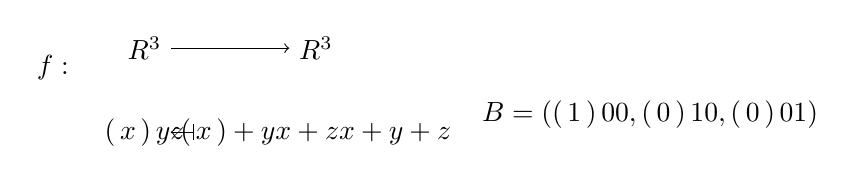
\begin{tikzpicture}[node distance=1mm]
    \node (functionName) at (0, -0.5) {$f:$};

    \node[above right = -0.3cm and 0.5cm of functionName] (domain) {$\mathbb{R}^3$};
    \node[right = 1.5cm of domain] (codomain) {$\mathbb{R}^3$};
    \node[below right = 0.1mm and 5cm of functionName] (Basis) {$B = \left(\begin{pmatrix} 1 \\ 0 \\ 0 \end{pmatrix} , \begin{pmatrix} 0 \\ 1 \\ 0 \end{pmatrix} , \begin{pmatrix} 0 \\ 0 \\ 1 \end{pmatrix}\right)$};
    \node[below = 5mm of domain] (element) {$\begin{pmatrix} x \\ y \\ z \end{pmatrix}$};
    \node at (element-|codomain) (image) {$\begin{pmatrix} x + y \\ x + z \\ x + y + z\end{pmatrix}$};
    \draw[->] (domain) -- (codomain);
    \draw[|->] (element) -- (image) ;
\end{tikzpicture}\\
$A = Mat{B}(f)$ so $A$ invertible $\Longleftrightarrow$ $f$ is an automorphism \\
so $A^{-1} = Mat{B}(f^{-1})$ \\
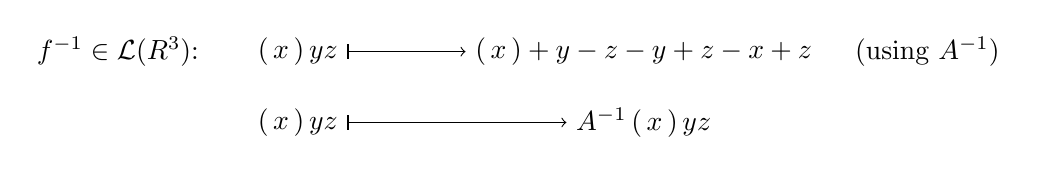
\begin{tikzpicture}[node distance=1mm]
    \node (functionName) at (0, -0.5) {$f^{-1} \in \mathcal{L}(R^3)$:};

    \node[right = 0.5cm of functionName] (domain) {$\begin{pmatrix} x \\ y \\ z \end{pmatrix}$};
    \node[right = 1.5cm of domain] (codomain) {$\begin{pmatrix} x + y  - z \\ -y + z \\ - x + z  \end{pmatrix}$};
    \node[right = 3mm of codomain] (using) {(using $A^{-1}$)};
    \node[below = 3mm of domain] (element) {$\begin{pmatrix} x \\ y \\ z \end{pmatrix}$};
    \node at (element-|codomain) (image) { $A^{-1} \begin{pmatrix} x \\ y \\ z \end{pmatrix}$};
    \draw[|->] (domain) -- (codomain);
    \draw[|->] (element) -- (image) ;
\end{tikzpicture}\\
\paragraph{Example 2}
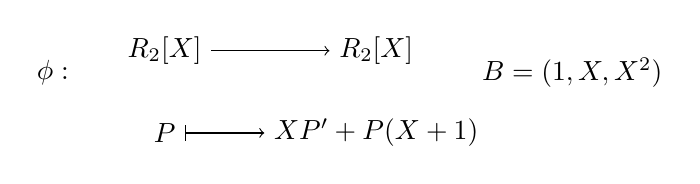
\begin{tikzpicture}[node distance=1mm]
    \node (functionName) at (0, -0.5) {$\phi:$};

    \node[above right = -0.3cm and 0.5cm of functionName] (domain) {$\mathbb{R}_2[X]$};
    \node[right = 1.5cm of domain] (codomain) {$\mathbb{R}_2[X]$};
    \node[right = 5cm of functionName] (Basis) {$B = (1, X,X^2)$};
    \node[below = 5mm of domain] (element) {$P$};
    \node at (element-|codomain) (image) {$XP'+P(X+1)$};
    \draw[->] (domain) -- (codomain);
    \draw[|->] (element) -- (image) ;
\end{tikzpicture}\\
So we have:
$\phi(1) = 1$ and $\phi(X) = 2X + 1$ and $\phi(X^2) = 3X^2 + 2X + 1$ \\
So:
$A = Mat_ {B}(\phi) = \begin{pmatrix} (\phi(1) & \phi(X) & \phi(X^2))\\1 & 1 & 1 \\ 0 & 2 & 2 \\ 0 & 0 & 3 \end{pmatrix} \begin{matrix}
    \\1 \\ X \\ X^2
\end{matrix}$ \\ an invertible matrix (upper right triangle with non zero diagonal coefficient\\
We have to find $A^{-1}$ to find $\phi^{-1}$ \\
\begin{align*}
     \left( \begin{array}{ccc|ccc}
        \circled{1} & 1 & 1 & 1 & 0 & 0 \\
        0 & \circled{2} & 2 & 0 & 1 & 0 \\
        0 & 0 & \circled{3} & 0 & 0 & 1 \\
    \end{array}\right)  \begin{matrix}3R_1 - R_3 \\ R_2 - 2R_3 \\ R_3\end{matrix}
     \Longleftrightarrow &
    \left( \begin{array}{ccc|ccc}
        3 & 3 & 0 & 3 & 0 & -1 \\
        0 & 6 & 0 & 0 & 3 & -1 \\
        0 & 0 & 3 & 0 & 0 & 1 \\
    \end{array}\right) \begin{matrix} 2R_1-R_2 \\ R_2 \\ R_3 \end{matrix}  \\ 
    \Longleftrightarrow&
    \left( \begin{array}{ccc|ccc}
        6 & 0 & 0 & 6 & -3 & 0 \\
        0 & 6 & 0 & 0 & 3 & -2 \\
        0 & 0 & 3 & 0 & 0 & 1 \\
    \end{array}\right) \begin{matrix} \frac{1}{6}R_1 \\ \frac{1}{6}R_2 \\ \frac{1}{3}R_3 \end{matrix}  \\
    \Longrightarrow&  \left[ Mat_{B}(\phi) \right]^{-1} = \begin{pmatrix} 1 & -\frac{1}{2} & 0 \\ 0 & \frac{1}{2} & -\frac{1}{3} \\ 0 & 0 & \frac{1}{3} \end{pmatrix} \\
    \Longrightarrow& \left[ Mat_{B}(\phi) \right]^{-1} = \frac{1}{6} \begin{pmatrix} 6 & -3 & 0 \\ 0 & 3 & -2 \\ 0 & 0 & 2 \end{pmatrix} \\
\end{align*}
Now find $Q \in \mathbb{R}_2[X], \phi(Q)(X) = 1 + (X-1)^2$ \\
$\phi^{-1}(1 + (X-1)^2)$ ? we use the matrix to find the coordinates: $1+ (X-1)^2 = 2 -2X +X^2$ \\
\[\frac{1}{6} \begin{pmatrix} 6 & -3 & 0 \\ 0 & 3 & -2 \\ 0 & 0 & 2 \end{pmatrix} \cdot \begin{pmatrix} 2 \\ -2 \\ 1 \end{pmatrix}_B = \frac{1}{6} \begin{pmatrix} 18 \\ -8 \\ 2 \end{pmatrix}_B = \begin{pmatrix} 3 \\ -\frac{4}{3} \\ \frac{1}{3} \end{pmatrix}_B\]
\[ \exists ! Q \in \mathbb{R}[X], \phi(Q) = \mathbb{R} \quad Q(X) = 3 - \frac{4}{3}X - \frac{1}{3}X^2\]
\end{document}